\documentclass[11pt]{article}
\usepackage[letterpaper,margin=1in]{geometry}
\usepackage{amsmath,amssymb,amsfonts}
\usepackage{booktabs,tabularx,array,multirow}
\usepackage{graphicx,float,caption}
\usepackage{xcolor}
\usepackage{microtype}
\usepackage{enumitem}
\usepackage{cite}
\usepackage[hidelinks]{hyperref}
\usepackage{url}
\usepackage{xspace}

{\color{red}% BEGIN SECOND-ROUND REVISION
% Toggle this flag in the marked copy. The clean manuscript keeps revised
% passages black while the response-package copy renders them in red.
\newif\ifshowrevisions
\showrevisionsfalse
\ifshowrevisions
  \newcommand{\revised}[1]{\textcolor{red}{#1}}
\else
  \newcommand{\revised}[1]{#1}
\fi

}% END SECOND-ROUND REVISION
\definecolor{cbadred}{HTML}{C0392B}
\definecolor{modelblue}{HTML}{2874A6}
\definecolor{softgray}{HTML}{F3F5F7}
\newcommand{\method}{MD-CBAD-DQN\xspace}
\newcommand{\R}{\mathbb{R}}
\DeclareMathOperator{\clip}{clip}

{\color{red}% BEGIN SECOND-ROUND REVISION
\title{\textbf{Counterfactual Full-Action Bellman Supervision for Temporally Coupled Satellite-Ground Scheduling}}
}% END SECOND-ROUND REVISION
\author{
Bocheng Yang$^{1}$, Lujie Zheng$^{1}$, Jian Liu$^{1,2,*}$, and Bo Chen$^{1,*}$\\[3pt]
\small $^{1}$School of Aerospace, Harbin Institute of Technology (Shenzhen), Shenzhen 518055, China\\
\small $^{2}$Guangxi Key Laboratory of Precision Navigation Technology and Application,\\[-2pt]
\small Guilin University of Electronic Technology, Guilin 541004, China\\
\small $^{*}$Correspondence: liujian2024@hit.edu.cn; hitchenbo@hit.edu.cn
}
\date{}

\begin{document}
\emergencystretch=2em
\maketitle
\input{generated/reviewer_macros.tex}

\begin{abstract}
{\color{red}% BEGIN SECOND-ROUND REVISION
Satellite-ground scheduling is temporally coupled because a locally inexpensive action can consume resources needed by later tasks. A standard deep Q-network (DQN) trains only the executed action even when an analytical model can evaluate every one-step alternative. We introduce \method, which constructs Bellman targets for all three processing modes and distills their centered within-state advantages. Training therefore evaluates the two unchosen modes, whereas deployment uses no preview. The factual target and loss term are retained, while the auxiliary gradient changes the total update. We evaluate a fully specified synthetic, soft-constrained single-satellite simulator using \IndependentModelSeeds{} model seeds and shared held-out traces. Against standard DQN, \method reduced mean composite cost by \PhysicalCBADMinPct--\PhysicalCBADMaxPct across five fully coupled regimes under the prespecified paired common-random-number analysis. Uncentered full-action Bellman supervision matched CBAD within uncertainty, whereas removing the bootstrap weakened the benefit. Double-CBAD also had lower nominal mean cost than Double DQN, although its family-adjusted sign test did not cross 0.05. Exact planning reduced mean cost from 99.33 at one step to 89.35 at six steps while increasing mean action-selection time from 0.13 to 41.60 ms. Both principal learned policies reached zero remaining energy in some episodes, so the results establish neither hard-constrained deployability nor validity for flight dynamics outside the defined simulator.
}% END SECOND-ROUND REVISION
\end{abstract}

\noindent\textbf{Keywords:} satellite edge computing; task scheduling; model-driven reinforcement learning; counterfactual supervision; Bellman advantage distillation.

\begin{figure}[!htbp]
\centering
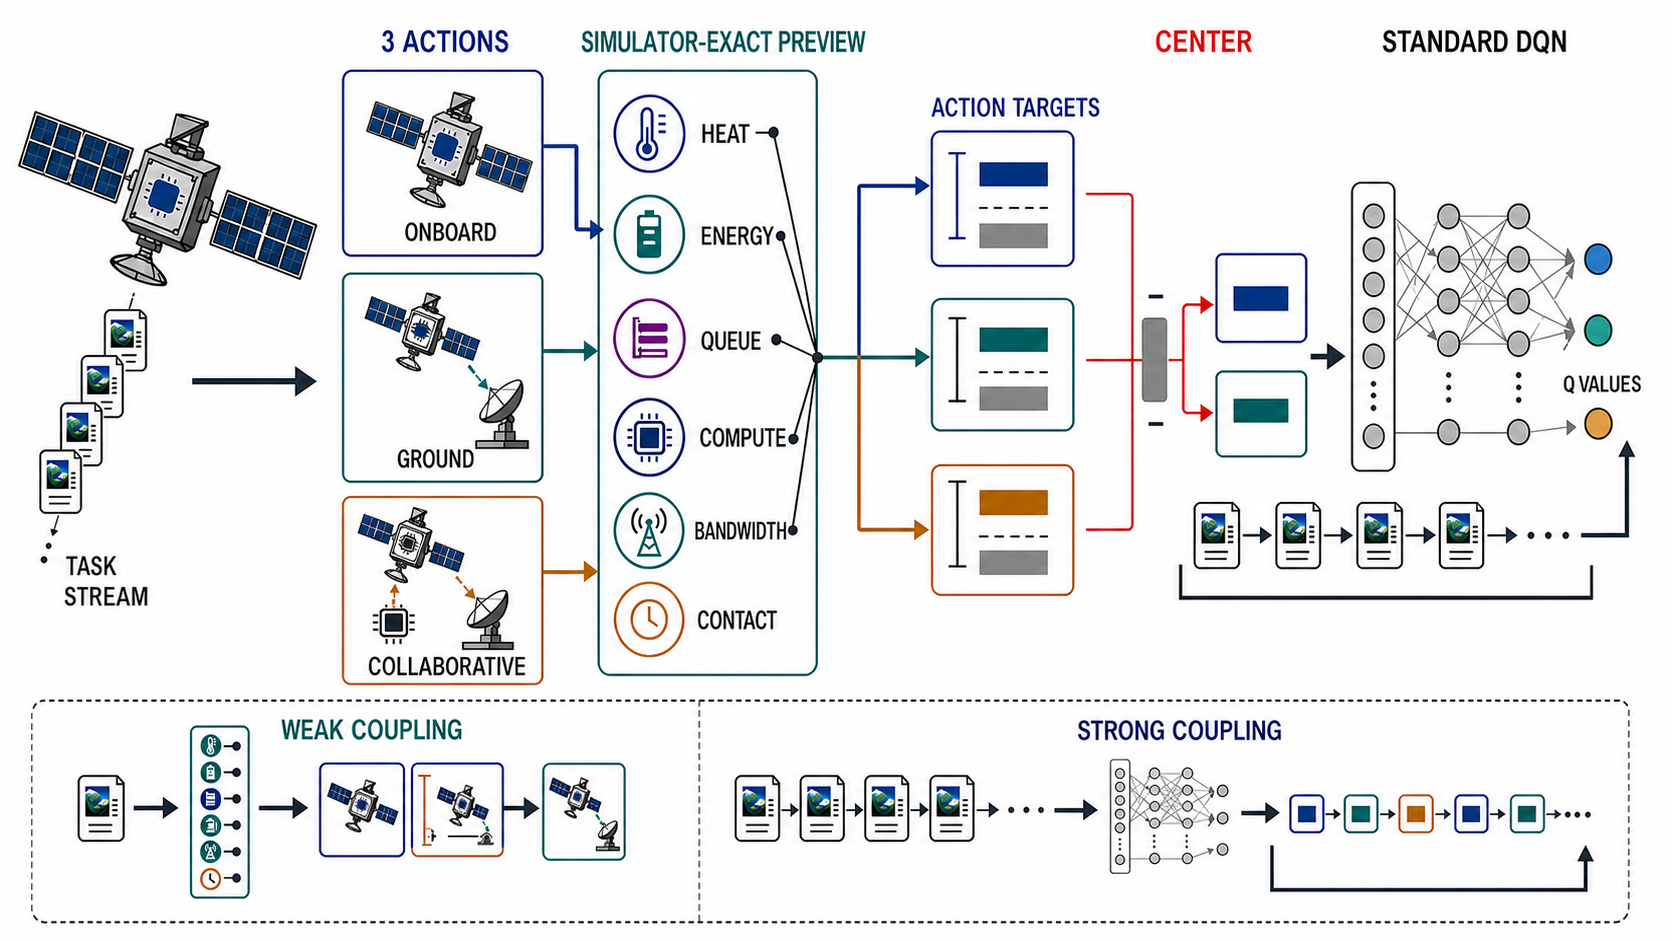
\includegraphics[width=0.98\textwidth,height=0.42\textheight,keepaspectratio]{figures/ai/fig_graphical_abstract_simulator_exact_arial.png}
\caption{Graphical overview of \method. Simulator-exact analytical previews expose the immediate cost and six post-action resources for all three scheduling actions. Centering the resulting Bellman targets isolates action-relative supervision. The factual standard-DQN target and loss term are retained, and the auxiliary loss contributes an additional gradient during training. The illustration is conceptual and encodes no quantitative results.}
\label{fig:graphical}
\end{figure}

\section{Introduction}

Earth-observation and communication satellites increasingly execute perception and decision workloads in orbit. Compact networks can reduce downlink demand and response latency under constrained onboard resources~\cite{9925218,10107454,10378728,10440355,10423050}. Yet onboard execution consumes heat, energy, and compute capacity, while ground offloading consumes contact time and bandwidth. A scheduler must therefore choose among onboard execution, complete offloading, and collaborative preprocessing.

{\color{red}% BEGIN SECOND-ROUND REVISION
Existing schedulers optimize constellation coordination, observation plans, service placement, deadlines, makespan, or energy use~\cite{RN8,RN10,RN20,RN22,RN23,RN27,RN28}. The present decision instead changes six resources that persist across task arrivals. These resources are heat, energy, queue occupancy, compute utilization, bandwidth, and remaining contact. Consider two consecutive tasks. Onboard execution may be cheapest for the first task, yet its heat and energy use can make ground or collaborative processing preferable when the second task arrives. The scientific question is therefore whether model-defined one-step alternatives can teach a policy these action gaps without requiring preview at deployment.
}% END SECOND-ROUND REVISION

Standard DQN~\cite{mnih2015human,watkins1992q} learns one Bellman target from each factual tuple $(s_t,a_t,r_t,s_{t+1})$. Here, the resource equations can also evaluate every unexecuted action without advancing the environment or revealing later tasks. The unresolved question is how to use these simulator-exact alternatives while preserving a controlled standard-DQN comparison. Absolute counterfactual targets provide more supervision, but their common state-value offset does not affect action selection.

We address this question with \method. The method previews every action, forms standard target-network Bellman targets, and centers predicted and target values within each state. It then distills the resulting action advantages while the factual Huber loss anchors the absolute Q scale. Counterfactual previews are restricted to training.

Our contributions are:

\begin{enumerate}[leftmargin=1.6em]
    \item We formulate three satellite-ground processing modes as a 21-dimensional sequential problem and derive coupled heat, energy, latency, and transmission descriptors from common task primitives.
{\color{red}% BEGIN SECOND-ROUND REVISION
    \item We introduce a counterfactual full-action Bellman objective whose centered implementation supervises the action gaps that determine scheduling decisions.
    \item We evaluate this objective against a strictly matched standard-DQN backbone. Component controls support Bellman-supervised full-action labels but do not isolate centering as necessary. Coupling controls, a Double-DQN pair, and finite-horizon planners further bound the result.
}% END SECOND-ROUND REVISION
\end{enumerate}

\section{Related Work and Novelty Positioning}

\subsection{Satellite-ground scheduling}

{\color{red}% BEGIN SECOND-ROUND REVISION
Satellite schedulers cover constellation coordination, observation planning, service placement, and energy-aware offloading~\cite{RN8,RN10,RN20,RN22,RN23,RN27,RN28}. Our setting combines an explicit cost for every action with resource carryover between task arrivals. The one-step objective is therefore observed rather than hidden. Learning is justified only when present actions change future feasibility.
}% END SECOND-ROUND REVISION

\subsection{Model use and counterfactual learning}

{\color{red}% BEGIN SECOND-ROUND REVISION
Dyna established predicted experience for value learning and planning~\cite{sutton1991dyna}, and model-based acceleration has also been used to supplement deep Q-learning with locally fitted dynamics~\cite{gu2016continuous}. Counterfactual data fusion and causal augmentation construct transitions under structural assumptions~\cite{forney2017counterfactual,armengol2024caiac}. Counterfactual credit assignment instead separates action influence from future randomness~\cite{mesnard2021counterfactual}. Recent work also studies multi-action generative interfaces and joint quantities across action outcomes~\cite{kaya2026joint}. Counterfactual information and model-assisted Q-learning are therefore not new by themselves.
}% END SECOND-ROUND REVISION

{\color{red}% BEGIN SECOND-ROUND REVISION
Advantage learning widens action gaps through modified operators~\cite{bellemare2016gap}, whereas \method retains the chosen DQN Bellman operator and adds a supervised action-gap loss. Unlike Dyna-style replay synthesis, the method inserts no modeled transition into replay. Unlike model-based acceleration through local rollouts, it uses one analytical outcome for every discrete action only inside an auxiliary target. The component study below directly compares centered Bellman advantages with uncentered full-action Q targets and centered immediate-cost targets. Our novelty claim is consequently narrow. We claim the evaluated full-action Bellman auxiliary design and its scheduling application, not counterfactual simulation, model-assisted Q-learning, advantage learning, or centering in general.
}% END SECOND-ROUND REVISION

\section{System Model and Immediate-Cost Quantification}
\label{sec:system}

At task arrival $t$, a satellite selects one of three actions:
\begin{equation}
\mathcal A=\{\alpha_s,\alpha_g,\alpha_{s\&g}\},
\end{equation}
where $\alpha_s$ executes onboard and downlinks the result, $\alpha_g$ downlinks the complete input for ground execution, and $\alpha_{s\&g}$ performs onboard preprocessing followed by ground execution.

\begin{figure}[H]
\centering
\includegraphics[width=0.98\textwidth,height=0.42\textheight,keepaspectratio]{figures/ai/fig_system_modes_arial.png}
\caption{Three satellite-ground processing pathways. Each arriving task is executed onboard, transferred for ground execution, or preprocessed collaboratively before ground completion. The analytical transition model returns the immediate cost and the post-action heat, energy, queue occupancy, compute utilization, bandwidth, and remaining contact.}
\label{fig:system}
\end{figure}

\subsection{Implemented immediate-cost model}

The revised experiments use the dimensionless linear cost implemented by the physical-consistency simulator. Let $x_k$ denote the 15 task descriptors in Table~\ref{tab:state_dictionary}. Each descriptor is normalized as
\begin{equation}
\bar x_k=\clip(x_k/s_k,0,1.5),
\end{equation}
where $s_k$ is the corresponding scale. For inherited normalized bandwidth $b$, the available return rate is $R(b)=2.2+217.8b$ Mbit s$^{-1}$. The three action latencies are
\begin{align}
L_s&=x_3+1000x_6/R(b),\notag\\
L_g&=x_8+1000x_9/R(b),\notag\\
L_{s\&g}&=1000x_{12}/4+x_{13}+1000x_{15}/R(b).
\label{eq:latencies}
\end{align}
The implemented immediate costs are
\begin{align}
c_s^{imm}={}&0.70\bar x_1+0.65\bar x_2+0.00045L_s+0.55\bar x_5
+0.35\bar x_6+0.35h+0.12(1-e),\notag\\
c_g^{imm}={}&0.45\bar x_7+0.00045L_g+0.55\bar x_9
+0.35(0.28-\tau)_+,\notag\\
c_{s\&g}^{imm}={}&0.55(\bar x_{10}+\bar x_{11})+0.55\bar x_{14}
+0.00045L_{s\&g}+0.45\bar x_{15}\notag\\
&+0.18h+0.12q+0.18(0.22-\tau)_+.
\label{eq:implemented_costs}
\end{align}
Here $h$, $e$, $q$, and $\tau$ are inherited heat, remaining energy, queue occupancy, and contact duration. The weights are fixed simulator assumptions rather than fitted mission utilities. They are applied identically during training, counterfactual preview, MPC evaluation, and deployment evaluation. Automated tests reproduce Eq.~\eqref{eq:implemented_costs} from the 15 raw descriptors and compare it with all three code outputs.

\begin{table}[H]
\centering
\caption{Implemented 15-dimensional task descriptor dictionary. The six appended resource coordinates are $h$, $e$, $q$, compute utilization $u$, bandwidth $b$, and contact duration $\tau$.}
\label{tab:state_dictionary}
\resizebox{\textwidth}{!}{\input{generated/table_state_dictionary.tex}}
\end{table}

\subsection{Physically coupled task and communication generator}

The revised simulator does not sample heat, workload, data volume, and latency independently. It first draws correlated latent variables $(v_t,w_t)$ with correlation parameter 0.68 and maps them through a logistic transform to raw data volume $D_t\in[8,64]$ Mbit and workload $W_t\in[0.25,4.0]$ GFLOP. Result and collaborative-feature volumes are
\begin{equation}
D_t^{res}=r_tD_t,\quad r_t\in[0.01,0.05],\qquad
D_t^{feat}=f_tD_t,\quad f_t\in[0.08,0.30].
\end{equation}
The implementation enforces $D_t^{res}\le D_t^{feat}\le D_t$. A workload-dependent fraction $p_t\in[0.20,0.45]$ is processed onboard in the collaborative mode. Given onboard and ground rates $R_s=4$ and $R_g=80$ GFLOP s$^{-1}$, processing time is derived as $W/R$, rather than sampled separately. Compute power rises monotonically from 4 to 20 W with workload; compute heat is 0.78 times compute energy. Transmission time is data volume divided by the effective return rate
\begin{equation}
R_t^{link}=2.2+217.8b_t\quad\text{Mbit s}^{-1},
\end{equation}
and transmission heat is 0.55 times transmit energy. These values are engineering envelopes, not fitted flight distributions. Their scale is consistent with the range of modern SmallSat computing-system power reported by NASA and with NASA ground-network examples spanning 2.2 Mbit s$^{-1}$ S-band to 220 Mbit s$^{-1}$ X-band returns~\cite{nasa2026avionics,nasa2026ground}. The bounded data-reduction factors represent the bandwidth-reduction role of onboard image compression, not a claim about one instrument-specific codec~\cite{ccsds122}. Table~\ref{tab:parameters} states every implemented assumption.

\begin{table}[H]
\centering
\caption{Physical primitives and provenance of the revised simulator. Values define a transparent engineering envelope; they are not presented as a fitted flight distribution.}
\label{tab:parameters}
\resizebox{\textwidth}{!}{\input{generated/table_parameter_provenance.tex}}
\end{table}

An automated audit generated \PhysicalAuditTasks{} tasks before training. All values were finite and positive, all data-flow inequalities held, and the empirical raw-data--workload correlation was \PhysicalCorrDataWork. Figure~\ref{fig:physical} shows the resulting dependence structure. Constant-rate columns have zero variance and are therefore excluded from correlation coefficients.

\begin{figure}[H]
\centering
\includegraphics[width=0.98\textwidth]{figures/fig_physical_generator.pdf}
\caption{Physical-consistency audit of the revised generator. (a) A legibility sample of 2,000 of 20,000 tasks; color encodes heat derived from compute energy. (b) Correlations computed from all 20,000 tasks. No fitted flight distribution is implied.}
\label{fig:physical}
\end{figure}

{\color{red}% BEGIN SECOND-ROUND REVISION
\subsection{Complete stochastic generator and action-load specification}
\label{sec:complete_simulator}

For independent reconstruction, this subsection states the remaining simulator functions that enter the transition. Let $u_D,\epsilon_W\sim\mathcal N(0,1)$ independently, $u_W=0.68u_D+\sqrt{1-0.68^2}\epsilon_W$, and $g(u)=[1+\exp(-1.55u)]^{-1}$. Nominal raw volume and workload are
\begin{equation}
D=8+56g(u_D)\ {\rm Mbit},\qquad W=0.25+3.75g(u_W)\ {\rm GFLOP}.
\label{eq:primitive_generator}
\end{equation}
The burst interval occupies indices $\lfloor T/3\rfloor$ through $\lfloor T/3\rfloor+\max(4,\lfloor T/4\rfloor)-1$ and multiplies both quantities by 1.45. With independent $U_r,U_f\sim\mathcal U(0,1)$,
\begin{align}
r&=0.01+0.04U_r,\qquad f=0.08+0.22\clip[0.65g(u_W)+0.35U_f,0,1],\notag\\
p&=0.20+0.25g(u_W),\qquad D^{res}=rD,\quad D^{feat}=fD,\quad W^{pre}=pW.
\label{eq:primitive_ratios}
\end{align}
Onboard and ground rates are 4 and 80~GFLOP~s$^{-1}$, respectively. Compute power is $P_c=4+16\clip(W/4.8,0,1)^{0.70}$~W, and transmit power is 6~W. Compute and transmit heat are 0.78 and 0.55 times their corresponding energy use. These definitions generate all 15 coordinates in Table~\ref{tab:state_dictionary}.

At reset, a single phase $\phi\sim\mathcal U(0,2\pi)$ generates the exogenous link trace
\begin{align}
\bar b_t&=\clip\left\{\kappa_b[0.62+0.23\sin(2\pi t/24+\phi)+\epsilon^b_t]-I_{link},0.12,1\right\},\notag\\
\bar\tau_t&=\clip\left\{0.55+0.35\sin(2\pi t/31+\phi/2)+\epsilon^\tau_t,0.08,1\right\},
\label{eq:link_trace}
\end{align}
where $\epsilon^b_t\sim\mathcal N(0,0.06^2)$, $\epsilon^\tau_t\sim\mathcal N(0,0.04^2)$, $\kappa_b$ is the sensitivity multiplier, and $I_{link}=0.22$ only in the link-limited regime. All episode tasks and link states are drawn at reset from one seeded NumPy generator.

The normalized action loads used in Eq.~\eqref{eq:transition} are stated here in action order $(\alpha_s,\alpha_g,\alpha_{s\&g})$:
\begin{align}
\widehat w&=(W,0.05W,W)/4.8,\qquad
\widehat Q=(x_1,0.20x_7,x_{10}+x_{11})/100,\notag\\
\widehat B&=(x_6,x_9,x_{15})/76.8,\notag\\
\Delta e&=\kappa_e\left(0.012+0.042\widehat w_1,
0.007+0.025\widehat B_2/b,
0.010+0.025\widehat w_3+0.018\widehat B_3/b\right),\notag\\
\Delta q&=\left(0.055\widehat w_1(1+u),
0.048\widehat B_2/b,
0.030(\widehat w_3+\widehat B_3/b)\right),\notag\\
\mu&=\left(0.030(1-u),0.035b\tau,0.032(1-0.5u)\right),\notag\\
\ell&=(0.02,0.18\widehat B_2,0.12\widehat B_3).
\label{eq:action_loads}
\end{align}
Here divisions by $b$ use $\max(b,0.1)$. The utilization targets in Eq.~\eqref{eq:transition} are $(\widehat w_1,0.10\widehat B_2,0.55\widehat w_3)$. Initial resources are $(h,e,q,u)=(0.22,0.88,0.12,0.18)$ except that energy-limited episodes use $e=0.62$ and thermal-stress episodes use $h=0.42$. Each episode terminates after exactly 64 executed actions; the terminal Bellman multiplier is zero. Energy and other resources remain soft-constrained clipped states, so reaching $e=0$ does not mask actions or terminate an episode.

}% END SECOND-ROUND REVISION
\section{Sequential Scheduling Formulation}
\label{sec:mdp}

\subsection{State and transition}

The normalized 21-dimensional state is
\begin{equation}
s_t=[x_t,z_t],\qquad z_t=[h_t,e_t,q_t,u_t,b_t,\tau_t],
\end{equation}
where $x_t\in\R^{15}$ contains the task inputs defined in Table~\ref{tab:state_dictionary}. The six resource variables denote normalized heat, remaining energy, queue occupancy, compute utilization, bandwidth, and contact duration.

Executing action $a_t$ changes resources before the next exogenous task arrives. The implemented transition is
\begin{align}
h_{t+1}&=\clip(0.86h_t+0.17c\widehat Q_t^{(a_t)},0,1.3),\notag\\
e_{t+1}&=\clip(e_t+0.006-c\Delta e_t^{(a_t)},0,1),\notag\\
q_{t+1}&=\clip(q_t+c(\Delta q_t^{(a_t)}-\mu_t^{(a_t)}),0,1.3),\notag\\
u_{t+1}&=\clip(0.68u_t+0.32c\widehat w_t^{(a_t)},0,1.2),\notag\\
b_{t+1}&=\clip(\bar b_{t+1}-c\ell_t^{(a_t)},0.08,1),\notag\\
\tau_{t+1}&=\clip(\bar\tau_{t+1}-0.10c\widehat B_t^{(a_t)},0.05,1).
\label{eq:transition}
\end{align}
{\color{red}% BEGIN SECOND-ROUND REVISION
Here $\widehat Q$, $\widehat w$, and $\widehat B$ are normalized action-specific heat, work, and data demands. The terms $\Delta e$, $\Delta q$, $\mu$, and $\ell$ are the deterministic resource-use, queue, service, and link-occupation functions defined in Eq.~\eqref{eq:action_loads}. Exogenous link variables $\bar b$ and $\bar\tau$ follow Eq.~\eqref{eq:link_trace} and are sampled before each episode. Coupling $c=0$ removes action-dependent carryover, $c=0.5$ weakens it, and $c=1$ defines full coupling.
}% END SECOND-ROUND REVISION

\subsection{Reward and standard DQN backbone}

The reward is the negative immediate cost plus post-decision feasibility penalties:
\begin{align}
r_t={}&-c_t^{imm}-c\big[12(h_{t+1}-0.78)_+ +15(0.18-e_{t+1})_+\notag\\
&+8(q_{t+1}-0.75)_+ +10\mathbf 1_{a_t\ne\alpha_s}(0.14-\tau_t)_+\big].
\label{eq:reward}
\end{align}
The DQN uses the unmodified factual target
\begin{equation}
y_t=r_t+\gamma(1-d_t)\max_{a'}Q_{\bar\theta}(s_{t+1},a'),
\label{eq:factual}
\end{equation}
and factual loss
\begin{equation}
L_{DQN}=\mathcal H\big(Q_\theta(s_t,a_t),y_t\big),
\end{equation}
where $\mathcal H$ denotes the Huber loss. The target network both selects and evaluates the maximizing action, as required by standard DQN.

\section{Model-Driven Counterfactual Bellman Advantage Distillation}
\label{sec:method}

The proposed method preserves the factual DQN target and factual loss term and adds one training-only auxiliary path. This path supplies targets for unexecuted actions and removes their shared within-state offset. The experiment evaluates this complete auxiliary objective rather than attributing performance to either operation in isolation.

\subsection{Side-effect-free full-action preview}

For every replayed factual state, the analytical transition evaluates each $a\in\mathcal A$:
\begin{equation}
(\tilde \ell_{t,a},\tilde z'_{t,a})=F_{preview}(x_t,z_t,a).
\end{equation}
{\color{red}% BEGIN SECOND-ROUND REVISION
Here $\tilde \ell_{t,a}$ contains the immediate cost and post-decision feasibility penalty for action $a$. The preview does not advance time, mutate state, alter trajectories, or consume random numbers. Before action selection it computes only the current-task cost and six post-action resources. The factual action is then executed once, after which the next exogenous task $x_{t+1}$ is revealed and the replay tuple is completed. During a later replay update, all alternatives reuse this observed next task and exogenous link trace. The counterfactual next state therefore replaces only the six endogenous resource coordinates:
}% END SECOND-ROUND REVISION
\begin{equation}
\tilde s'_{t,a}=[x_{t+1},\tilde z'_{t,a}].
\end{equation}
Evaluation and deployment never call the preview interface.

\subsection{All-action counterfactual Bellman targets}

The simulator-exact one-step outcome yields
\begin{equation}
\tilde y_{t,a}=-\tilde \ell_{t,a}+\gamma(1-d_t)
\max_{a'}Q_{\bar\theta}(\tilde s'_{t,a},a').
\label{eq:cf_target}
\end{equation}
The targets create no multi-step rollout and insert no counterfactual transition into replay. They are used only after state-wise centering in the complete method below.

\subsection{Centered advantage distillation}

Absolute targets in Eq.~\eqref{eq:cf_target} share a bootstrapped state-value offset. Deployment selects $\arg\max_a Q(s,a)$, so a common additive offset cannot change the action. We define predicted and target centered advantages as
\begin{align}
\widehat A_{t,a}&=Q_\theta(s_t,a)-\frac{1}{|\mathcal A|}\sum_jQ_\theta(s_t,j),\notag\\
\tilde A_{t,a}&=\tilde y_{t,a}-\frac{1}{|\mathcal A|}\sum_j\tilde y_{t,j}.
\label{eq:center}
\end{align}
The advantage and total losses are
\begin{align}
L_{adv}&=\frac{1}{|\mathcal A|}
\sum_{a\in\mathcal A}\mathcal H(\widehat A_{t,a},\tilde A_{t,a}),\notag\\
L_{CBAD}&=L_{DQN}+\lambda L_{adv}.
\label{eq:cbad}
\end{align}
The factual term anchors the absolute Q scale, while $L_{adv}$ teaches all action gaps. The only added algorithmic hyperparameter is $\lambda$.

\begin{figure}[H]
\centering
\includegraphics[width=0.98\textwidth,height=0.43\textheight,keepaspectratio]{figures/ai/fig_cbad_mechanism_simulator_exact_arial.png}
\caption{Training-only CBAD mechanism. The upper path retains the factual standard-DQN target and Huber loss. The lower path previews all three actions, constructs three Bellman targets, centers them within state, and distills their relative advantages. Both losses update the online Q-network; the target network is synchronized only at the shared fixed interval. Preview outputs are unavailable during evaluation and deployment.}
\label{fig:mechanism}
\end{figure}

\begin{figure}[H]
\centering
\fbox{\begin{minipage}{0.93\textwidth}
\textbf{Algorithm 1: Pure-DQN training with CBAD}
\begin{enumerate}[leftmargin=1.6em,itemsep=2pt,topsep=4pt]
\item Initialize uniform replay $\mathcal D$, online $Q_\theta$, and target $Q_{\bar\theta}\leftarrow Q_\theta$.
{\color{red}% BEGIN SECOND-ROUND REVISION
\item At each real step, observe $s_t$ and preview current-task outcomes $(\tilde \ell_{t,a},\tilde z'_{t,a})$ for all actions without side effects.
\item Select $a_t$ by the shared epsilon-greedy schedule and execute it once. After $x_{t+1}$ is revealed, store the factual tuple plus the previously computed previews.
}% END SECOND-ROUND REVISION
\item When an update is due, sample one uniform mini-batch, compute the factual loss, compute Eqs.~\eqref{eq:cf_target} and \eqref{eq:center}, and update $\theta$ using Eq.~\eqref{eq:cbad}.
\item Synchronize $Q_{\bar\theta}$ at the shared fixed interval.
\end{enumerate}
\end{minipage}}
\par\smallskip
\caption*{Training previews are never used for evaluation or deployment.}
\label{alg:cbad}
\end{figure}

\section{Experimental Design and Settings}
\label{sec:experiments}

\subsection{Design principles}

{\color{red}% BEGIN SECOND-ROUND REVISION
The design separates four questions. Standard DQN versus CBAD tests the complete centered counterfactual objective against an unchanged factual DQN backbone. An uncentered full-action Q auxiliary target and a centered immediate-cost auxiliary target distinguish state-wise centering and Bellman bootstrapping from the effect of supplying three labels per state. Double DQN and Double-CBAD test whether the auxiliary objective transfers when action selection and target evaluation are decoupled~\cite{vanhasselt2016double}. Coupling controls and planners with $H\in\{1,2,4,6\}$ test whether long-horizon learning remains useful as delayed resource effects and planning depth change.
}% END SECOND-ROUND REVISION

{\color{red}% BEGIN SECOND-ROUND REVISION
Standard DQN and CBAD share every component except the centered counterfactual auxiliary objective. They use the same input, network, replay, exploration, optimizer, update cadence, target synchronization, and gradient clipping. The full-action Q control applies the same auxiliary weight directly to the three uncentered Bellman targets. The immediate-advantage control centers the negative analytical one-step costs but omits their bootstrapped future values. Double DQN and Double-CBAD use online-network action selection with target-network evaluation in both factual and auxiliary Bellman targets. Dueling networks, prioritized replay, multi-step returns, noisy networks, and distributional value learning remain outside the comparison.
}% END SECOND-ROUND REVISION

{\color{red}% BEGIN SECOND-ROUND REVISION
The auxiliary weight was fixed before the physical-consistency experiment. A preceding calibration with model seeds 700--703 compared $\lambda\in\{0.1,0.3,1,3\}$. It selected $\lambda=0.3$ by maximizing the worst relative CBAD improvement across five fully coupled calibration regimes, with the smaller weight as the tie-break. Because that calibration used the preceding simulator version, it is a prior specification rather than evidence from the physical-consistency generator. The present confirmation and all new controls use seeds 800--819 without post hoc removal, replacement, or selection. Every learned policy was trained only on the nominal $c=1$ distribution.
}% END SECOND-ROUND REVISION

\begin{figure}[!htbp]
\centering
\includegraphics[width=0.98\textwidth,height=0.42\textheight,keepaspectratio]{figures/ai/fig_experiment_protocol_20seeds_arial.png}
{\color{red}% BEGIN SECOND-ROUND REVISION
\caption{Prespecification and confirmation protocol. A preceding-simulator calibration with four seeds selected $\lambda=0.3$ before the physical-consistency experiment. Twenty disjoint confirmation seeds, 800--819, are each evaluated on 20 shared held-out traces in seven regimes, with no physical-generator tuning or seed exclusion.}
\label{fig:protocol}
}% END SECOND-ROUND REVISION
\end{figure}

\subsection{Training configuration}

Each network has 21 inputs, hidden widths 128--128--64, ReLU activations, and three outputs. Every model receives 600 episodes of 64 tasks, totaling 38,400 real interactions. Fixed settings are $\gamma=0.97$, learning rate $3\times10^{-4}$, batch size 128, replay capacity 100,000, and gradient-norm limit 10. Training begins after 128 transitions and performs one update every four interactions. The checkpoint field \texttt{target\_interval=250} is evaluated only on update calls; because updates occur at interaction counts divisible by four, the two divisibility conditions coincide every 500 real interactions. Epsilon decreases linearly from 1 to 0.05 over 13,440 interactions.

The contextual bandit uses the same network, optimizer, exploration schedule, and interaction budget, with $\gamma=0$. It therefore learns the modeled one-step reward without a long-horizon Bellman term. Uniform replay stores only one-step factual transitions, with preview outputs attached as auxiliary training data.

All reported reviewer-revision experiments use the physically coupled generator described above. Link bandwidth and contact follow bounded noisy periodic traces generated at reset. Burst and thermal-stress episodes multiply raw data and workload by 1.45 during one contiguous interval; all dependent heat, energy, latency, and transmission quantities are recomputed from those primitives. The original independently sampled generator is retained only as a historical reproducibility mode and is not used for the revised results.

\subsection{Seven evaluation regimes}

The seven regimes separate coupling controls from fully coupled operating conditions:

\begin{enumerate}[leftmargin=1.6em]
    \item \textbf{Static ($c=0$):} removes action-dependent state transitions and delayed penalties.
    \item \textbf{Reduced coupling ($c=0.5$):} halves action-dependent resource effects.
    \item \textbf{Nominal ($c=1$):} matches the fully coupled training distribution.
    \item \textbf{Burst:} increases contiguous compute and thermal demand.
    \item \textbf{Link-limited:} reduces the available bandwidth trace by 0.22 before clipping.
    \item \textbf{Energy-limited:} lowers initial energy from 0.88 to 0.62.
    \item \textbf{Thermal-stress:} raises initial heat from 0.22 to 0.42 and includes the burst interval.
\end{enumerate}

The first two regimes control temporal coupling. The remaining five retain full coupling. Models trained at $c=1$ are transferred to both controls without retraining. Their control performance therefore measures a boundary and transfer mismatch, rather than the best policy attainable at lower coupling.

\subsection{Planning comparator, outcomes, and inference}

{\color{red}% BEGIN SECOND-ROUND REVISION
The deployment comparison includes immediate-cost argmin, a contextual bandit, a resource-threshold heuristic, standard DQN, \method, and exhaustive finite-horizon model-based planning. At every real decision, a planner enumerates all $3^H$ action sequences over the next $H$ known tasks and link states, minimizes discounted modeled cost with $\gamma=0.97$, executes only the first action, and replans. The primary table retains $H=4$. A separate nominal analysis evaluates $H\in\{1,2,4,6\}$ on 400 unique held-out traces and reports wall-clock cost per decision. Each planner is exact only for its stated perfect-forecast objective, not for the 64-step global problem. Fixed onboard and fixed ground policies serve as supplemental controls.
}% END SECOND-ROUND REVISION

{\color{red}% BEGIN SECOND-ROUND REVISION
The primary outcome is episode total cost. Secondary outcomes are immediate cost, delayed penalty, energy use, modeled latency, transmitted data, threshold-exposure steps, action fractions, planner wall-clock time, maximum heat, and minimum remaining energy. Every learned comparison uses a prespecified common-random-number block. The same model-seed number initializes network weights and controls episode task seeds, epsilon-exploration draws, and replay-index sampling in both algorithms. Trajectories may diverge after different greedy actions, but the matched seed remains the randomization block. Each seed is evaluated on the same 20 held-out traces and traces are averaged within seed, giving $n=20$ blocks per method. Two-sided 95\% percentile intervals use 10,000 paired bootstrap resamples with seed 20260829. Exact two-sided paired sign tests evaluate directional consistency, with Holm adjustment across the five fully coupled primary comparisons. We also report every seed-level difference and the leave-one-seed-out range. As a conservative sensitivity check, an independent-seed bootstrap resamples the two sets of 20 seed means separately and ignores the matching. Test traces and bootstrap draws are never treated as independent model replicates.
}% END SECOND-ROUND REVISION

\subsection{Prespecified sensitivity and training diagnostics}

{\color{red}% BEGIN SECOND-ROUND REVISION
Without retraining or selecting models, the nominal evaluation was repeated under eight profiles: the reference configuration; compute demand $\pm20\%$; raw data volume $\pm20\%$; energy use $+20\%$; heat load $+20\%$; and link capacity $-20\%$. Each profile retained the same 20 models and the same held-out trace namespace as the primary experiment, with Holm adjustment across the eight profiles. Training logs record every episode for all 20 seeds. Curves report a causal 25-episode moving mean and seed-level mean $\pm$ SD for total cost, energy use, latency, and delayed penalty. These diagnostics describe optimization trajectories; confirmation claims remain based on held-out traces.
}% END SECOND-ROUND REVISION

\subsection{Preview-model misspecification test}

{\color{red}% BEGIN SECOND-ROUND REVISION
The main experiment assumes that the analytical preview matches the simulator transition. To test this dependence, two additional CBAD model sets were trained without changing the factual environment or deployment evaluation. One set scaled preview one-step costs (immediate cost plus modeled penalty) and action-induced resource changes by 0.85, while the other used 1.15. Resource predictions were clipped to the same physical bounds after scaling around the current resource state. Each condition used the same 20 seeds, training budget, network, replay, and held-out trace namespace as the main experiment. These scales were fixed as symmetric stress tests and were not used for model selection.
}% END SECOND-ROUND REVISION

\subsection{Reproducible result entry point}

{\color{red}% BEGIN SECOND-ROUND REVISION
The core result entry point is \texttt{python -m md\_cbad\_dqn.reviewer\_experiments all --seeds 800-819 --resume}. The second-round controls use \texttt{python -m md\_cbad\_dqn.extended\_revision --seeds 800-819 --stage all --resume}. The first command trains or loads 60 primary learned-policy checkpoints plus 40 preview-error checkpoints. The second reuses standard DQN and CBAD and trains 80 component and Double-DQN checkpoints. It then evaluates six learned objectives, performs the independent-seed bootstrap, and evaluates four planning depths on 400 unique traces. The command \texttt{python -m md\_cbad\_dqn.transition\_audit} writes a fixed-seed, all-action example in which preview and executed costs and six resources agree coordinate by coordinate. Unit tests repeat this equality at both resource clipping boundaries and on the terminal step. Experiments used Python 3.13.9, NumPy 2.4.1, pandas 3.0.3, PyTorch 2.8.0 with CUDA 12.9, an NVIDIA GeForce RTX 5070 Ti, and Windows 11. Planning wall time was measured on a 12th Gen Intel Core i9-12900K with 24 logical processors after one untimed warm-up episode. Values report the mean over all timed decisions. Machine-readable metadata record the resolved variants, seeds, budgets, randomization blocks, result files, and runtime environment. Table scripts consume these files directly.
}% END SECOND-ROUND REVISION

\section{Results}
\label{sec:results}

\subsection{Physical consistency preserves the CBAD--DQN effect}

Table~\ref{tab:main} and Fig.~\ref{fig:seven} summarize the revised primary outcome. Values are mean $\pm$ SD across 20 independent model seeds after averaging 20 shared traces within each seed.

\begin{table}[H]
\centering
{\color{red}% BEGIN SECOND-ROUND REVISION
\caption{Episode total cost for deployment comparators under the physically coupled generator. All learned policies were trained only at nominal $c=1$; static and reduced-coupling rows are transfers without retraining. MPC-4 is exact only for its stated four-step perfect-forecast objective. Lower is better; bold marks the lowest mean.}
\label{tab:main}
}% END SECOND-ROUND REVISION
\resizebox{\textwidth}{!}{\input{generated/table_reviewer_main.tex}}
\end{table}

\begin{figure}[H]
\centering
\includegraphics[width=0.98\textwidth]{figures/fig_reviewer_primary.pdf}
{\color{red}% BEGIN SECOND-ROUND REVISION
\caption{Seven-regime performance under physically coupled task generation. Error bars are SD across 20 model-seed blocks after within-seed trace averaging. All learned models were trained at nominal $c=1$; control rows are transfers without retraining. The ordinate changes between panels and panel heights should not be compared directly.}
\label{fig:seven}
}% END SECOND-ROUND REVISION
\end{figure}

\begin{table}[H]
\centering
\caption{Seed-level primary inference for CBAD minus standard DQN in the five fully coupled regimes. Negative differences favor CBAD. The Holm family contains these five prespecified comparisons. LOO denotes the range of leave-one-seed-out mean differences.}
\label{tab:primary_inference}
\resizebox{\textwidth}{!}{\input{generated/table_primary_inference.tex}}
\end{table}

\begin{figure}[H]
\centering
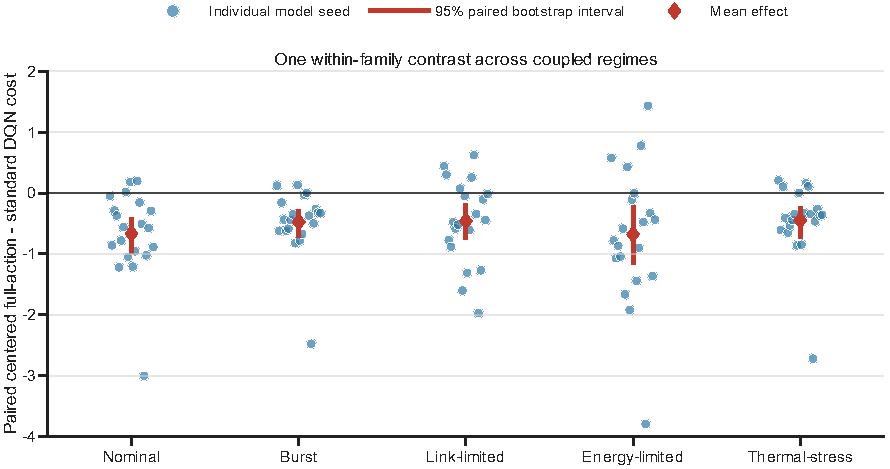
\includegraphics[width=0.98\textwidth]{figures/fig_seed_effects.pdf}
\caption{Paired total-cost differences for all 20 independent model seeds. Blue points show individual seed-level effects after averaging 20 shared traces. Red diamonds and vertical lines show mean differences and paired 95\% bootstrap intervals.}
\label{fig:seed_effects}
\end{figure}

{\color{red}% BEGIN SECOND-ROUND REVISION
\begin{table}[H]
\centering
\caption{Sensitivity of the primary CBAD--DQN comparison to ignoring the prespecified model-seed matching. The two groups of 20 seed means are resampled independently. These intervals quantify the loss of precision when the common-random-number blocks are discarded and are not the primary analysis.}
\label{tab:unpaired}
\resizebox{0.80\textwidth}{!}{\begin{tabular}{lrrr}
\toprule
Regime & Mean difference & Unpaired 95\% interval & Excludes zero \\
\midrule
Nominal & -0.67 & [-1.79, 0.46] & No \\
Burst & -0.48 & [-1.66, 0.73] & No \\
Link-limited & -0.46 & [-1.56, 0.60] & No \\
Energy-limited & -0.68 & [-1.80, 0.48] & No \\
Thermal-stress & -0.45 & [-1.62, 0.77] & No \\
\bottomrule
\end{tabular}}
\end{table}
}% END SECOND-ROUND REVISION

{\color{red}% BEGIN SECOND-ROUND REVISION
Across the five fully coupled regimes, \method had the lowest mean among all evaluated deployment methods and reduced standard-DQN cost by \PhysicalCBADMinPct--\PhysicalCBADMaxPct; every paired 95\% interval lay below zero. CBAD was lower for 16--18 of the 20 seed blocks in each regime, the largest Holm-adjusted sign-test value was \PrimaryHolmPMax, and every leave-one-seed-out mean remained negative (Table~\ref{tab:primary_inference}). Nominal mean cost decreased from \PhysicalNominalDQNCost for standard DQN to \PhysicalNominalCBADCost for CBAD. The independent-seed bootstrap was wider and excluded zero only in a subset of regimes (Table~\ref{tab:unpaired}). The direction therefore remains consistent, but the all-regime inferential statement depends on the prespecified common-random-number design. This replication changes both the task generator and model training, so it is a new physical-consistency experiment rather than a re-labeling of the earlier independent-range simulation.

At $c=0$, immediate argmin and MPC-4 were identical because actions had no delayed effect. At $c=0.5$, MPC-4 had the lowest mean. In contrast, CBAD outperformed MPC-4 in all five fully coupled regimes. Nominal MPC-4 cost was \MPCNominalCost, despite perfect four-task forecasts, and planning required \MPCNominalPlanningMs{} ms per decision on the evaluation workstation. This comparison alone does not identify the cause of the gap, so the planning-depth analysis below separates horizon and computation.

\subsection{Component controls identify Bellman bootstrapping, but not centering, as the supported distinction}

\begin{table}[H]
\centering
\caption{Nominal component and backbone controls. All models use 20 prespecified model-seed blocks, identical real-interaction budgets, and the same held-out traces. Full-action Q applies uncentered Bellman targets; immediate advantage centers analytical immediate costs without bootstrapping. Paired differences are relative to the matched reference named in the third column.}
\label{tab:extended_ablation}
\resizebox{\textwidth}{!}{\input{generated/table_extended_ablation.tex}}
\end{table}

Table~\ref{tab:extended_ablation} separates three explanations that the standard-DQN comparison cannot resolve. Uncentered full-action Q supervision reduced nominal cost by 1.29 relative to standard DQN, compared with 1.36 for CBAD; the direct CBAD-minus-full-action-Q difference was $-0.07$ with a paired 95\% interval of $[-0.32,0.20]$. Centering therefore showed no detectable increment under this design. The immediate-advantage control improved by 0.77 relative to standard DQN, but CBAD was lower by 0.58, with an interval of $[-1.00,-0.14]$. This pattern attributes the stronger effect to action-specific bootstrapped values rather than to three immediate labels alone. Double-CBAD was lower than Double DQN by 1.04, with an interval of $[-1.90,-0.38]$; however, the Holm-adjusted sign-test value was 0.059, so this transfer result is directional rather than confirmatory. These are fixed objective controls, not a post hoc search over alternative algorithms.

\subsection{Planning depth improves cost at a rapidly increasing computational price}

\begin{table}[H]
\centering
\caption{Nominal receding-horizon planning over 400 unique held-out traces. Each planner has perfect knowledge of the next $H$ tasks and exogenous link states and exactly enumerates $3^H$ sequences before every action. Runtime was measured on the same workstation and includes only action selection after environment construction.}
\label{tab:planner_depth}
\resizebox{0.85\textwidth}{!}{\input{generated/table_planner_depth.tex}}
\end{table}

Increasing planning depth reduced nominal mean cost from 99.33 at $H=1$ to 92.80, 90.83, and 89.35 at $H=2$, 4, and 6, respectively. The corresponding mean decision time increased from 0.13 ms to 0.49, 4.70, and 41.60 ms. The additional 1.48 cost-unit reduction from $H=4$ to $H=6$ therefore required an almost ninefold increase in action-selection time. Table~\ref{tab:planner_depth} should not be interpreted as a comparison with optimized approximate planning, dynamic programming, or mixed-integer methods. It quantifies only the exact-enumeration frontier implemented here, and the learned-policy comparison remains bounded to these transparent objectives.
}% END SECOND-ROUND REVISION

\begin{table}[H]
\centering
\caption{Engineering outcome decomposition for CBAD relative to standard DQN. Delta columns report CBAD minus DQN. Negative values denote lower use or cost. Low-energy steps count decisions with remaining energy below 0.18; they are soft-threshold exposures, not certified safety violations.}
\label{tab:engineering}
\small
\setlength{\tabcolsep}{4pt}
\input{generated/table_engineering_outcomes.tex}
\end{table}

Table~\ref{tab:engineering} separates the composite objective into its modeled consequences. Across the displayed regimes, CBAD reduced both immediate cost and delayed penalty, used slightly less modeled energy, and reduced modeled latency, while transmitting more data. The result is therefore a trade-off rather than a uniform reduction in every resource. The low-energy count is reported as threshold exposure because the simulator applies a soft penalty rather than a hard feasibility constraint. Both learned policies reached zero remaining energy and no evaluated episode was threshold-free, so these experiments do not establish hard-constrained deployability. Thermal-stress increases the initial heat and contiguous load, but the tested policies did not cross the heat threshold. It therefore probes elevated thermal load rather than certifying operation at a thermal safety boundary.

\subsection{Training diagnostics show stabilization of cost, energy, and latency}

\begin{figure}[H]
\centering
\includegraphics[width=0.98\textwidth]{figures/fig_training_diagnostics.pdf}
\caption{Training diagnostics for standard DQN and \method. Lines are means across 20 model seeds after a causal 25-episode moving average; shaded regions are $\pm$1 SD. Curves describe the training distribution and are not used as independent test observations.}
\label{fig:training}
\end{figure}

All four logged quantities declined rapidly during the first approximately 220 episodes and then fluctuated around a stable range (Fig.~\ref{fig:training}). Across seeds and episodes 501--600, CBAD averaged \LateCBADCost{} total cost, \LateCBADEnergy{} normalized energy use, \LateCBADLatency{} s latency, and \LateCBADPenalty{} delayed penalty, compared with \LateDQNCost, \LateDQNEnergy, \LateDQNLatency{} s, and \LateDQNPenalty{} for standard DQN. These curves answer the optimization question without reintroducing the undefined ``accuracy'' metric. They show empirical stabilization, not mathematical convergence.

\subsection{The result is robust within the tested parameter envelope}

\begin{table}[H]
\centering
\caption{Prespecified parameter sensitivity for CBAD minus standard DQN. Negative differences favor CBAD; $n=20$ independent paired model seeds in each profile. Holm adjustment covers the eight displayed profiles.}
\label{tab:sensitivity}
\resizebox{0.84\textwidth}{!}{\input{generated/table_sensitivity.tex}}
\end{table}

\begin{figure}[H]
\centering
\includegraphics[width=0.98\textwidth]{figures/fig_sensitivity_planning.pdf}
\caption{Parameter robustness and planning boundary. (a) Mean paired CBAD--DQN differences with 95\% paired bootstrap intervals. (b) Immediate, four-step rolling, and learned scheduling across coupling and stress regimes.}
\label{fig:sensitivity}
\end{figure}

The CBAD--DQN interval remained below zero in all eight profiles, with relative reductions from \SensitivityMinPct{} to \SensitivityMaxPct. The largest tested effect occurred when raw data volume decreased by 20\%, whereas the smallest occurred when it increased by 20\%. This analysis supports robustness only within these prespecified one-factor envelopes; it does not validate arbitrary hardware or mission distributions.

\subsection{Moderate preview error preserves a bounded benefit}

\begin{table}[H]
\centering
\caption{Effect of training-time preview misspecification. Differences are relative to the same standard-DQN models evaluated in the factual simulator. Scaling applies only to CBAD's training-only preview cost and action-induced resource changes.}
\label{tab:preview_mismatch}
\resizebox{\textwidth}{!}{\input{generated/table_preview_mismatch.tex}}
\end{table}

Table~\ref{tab:preview_mismatch} tests whether the auxiliary signal remains useful when its modeled one-step consequences are uniformly under- or over-scaled by 15\%. Both misspecified model sets retained negative mean differences and paired intervals below zero in all five regimes; their Holm-adjusted sign-test values were at most \MismatchHolmPMax. The 1.15 scale attenuated the mean benefit in four regimes, whereas the 0.85 scale produced effects close to the simulator-exact preview. This test does not represent arbitrary structural or action-specific error, but it separates simulator-internal exactness from moderate uniform calibration error and shows that the reported advantage survives this fixed perturbation.

\subsection{The learned policy adapts its action mix}

CBAD did not collapse to one processing mode. It increased onboard execution under link limitation and shifted toward ground or collaborative execution as the inherited state permitted. These action fractions are descriptive consequences of the learned policy, not additional inferential endpoints.

\begin{figure}[H]
\centering
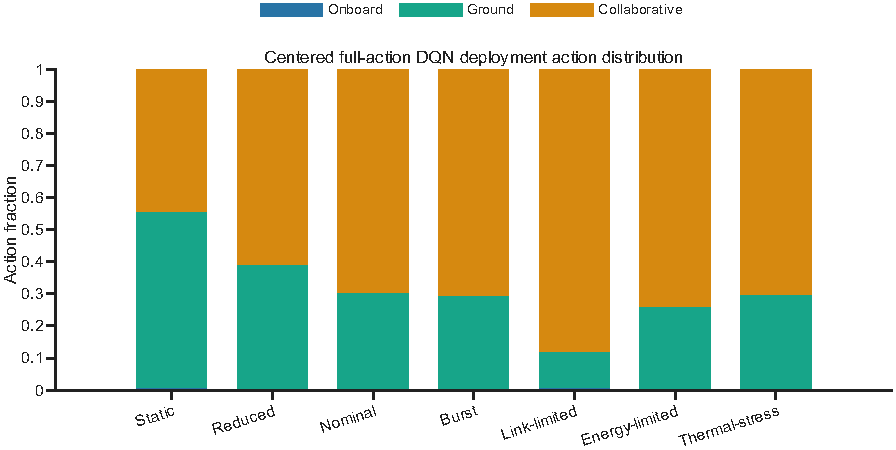
\includegraphics[width=0.90\textwidth]{figures/fig_reviewer_actions.pdf}
\caption{Mean deployment action fractions for \method under the physically coupled generator.}
\label{fig:actions}
\end{figure}

\section{Discussion and Limitations}

{\color{red}% BEGIN SECOND-ROUND REVISION
The revised evidence supports full-action Bellman auxiliary supervision against a strictly matched standard-DQN backbone across five fully coupled regimes. The centered CBAD form did not separate from its uncentered full-action Q control, so the present data do not attribute the gain specifically to centering. By contrast, the smaller immediate-advantage effect supports retaining action-specific future values. The Double-DQN pair was directionally consistent but not confirmatory after family adjustment. RL is not required for the static control, where immediate minimization is exact after action-dependent carryover is removed.
}% END SECOND-ROUND REVISION

{\color{red}% BEGIN SECOND-ROUND REVISION
The planning-depth comparison bounds the motivation more directly. Increasing $H$ from four to six reduced mean cost by 1.48 but multiplied decision time by 8.9, exposing a diminishing-return frontier within exact enumeration. It still does not establish the best horizon or compare against approximate tree search, mixed-integer programming, or dynamic programming with discretized resources. We therefore claim an advantage only over the reported exact finite-horizon objectives, not over planning or traditional optimization in general.
}% END SECOND-ROUND REVISION

{\color{red}% BEGIN SECOND-ROUND REVISION
The matched DQN backbone remains an attribution design rather than a broad reinforcement-learning benchmark. Double DQN is included as one prespecified stronger target construction and receives its own matched Double-CBAD arm. Dueling networks, prioritized replay, multi-step returns, noisy networks, and distributional value learning remain untested. Accordingly, the evidence does not establish superiority over every enhanced value-learning method.
}% END SECOND-ROUND REVISION

The new generator removes internally contradictory independent samples by deriving heat, energy, latency, and transmitted volume from common primitives. NASA and CCSDS sources bound selected engineering assumptions, while automated checks enforce data-flow inequalities. Nevertheless, the joint distribution is synthetic rather than fitted to mission telemetry. NASA itself cautions that component performance is mission-specific~\cite{nasa2026soa}. The sensitivity study covers only prespecified one-factor changes, not simultaneous uncertainty or structural model error.

{\color{red}% BEGIN SECOND-ROUND REVISION
Matched training components attribute the simulator-level comparisons to the stated objective changes, but external validity remains limited. ``Simulator-exact'' means one-step equality only with the specified deterministic program; it does not imply physical fidelity to a spacecraft. The topology remains one satellite and one ground path, the action space contains three modes, the utility weights are not mission-fitted, and inference remains simulation-based. Both principal learned policies reach zero remaining energy in some episodes because feasibility is represented by a soft penalty. Future work should impose action masking or constrained control, use flight or hardware-in-the-loop traces, expand to multiple satellites and contacts, and compare scalable approximate planning.
}% END SECOND-ROUND REVISION

\section{Conclusion}

{\color{red}% BEGIN SECOND-ROUND REVISION
We introduced \method to exploit one-step analytical resource models while retaining the factual DQN loss. In the defined synthetic soft-constrained simulator, CBAD had lower paired mean cost than standard DQN across five fully coupled regimes. Component controls localize the supported contribution to full-action Bellman supervision rather than centering alone; the matched Double-DQN result is directional after multiplicity control. Planning depths from one to six steps expose the cost of stronger exact look-ahead. The evidence establishes a simulator-level training-objective result, not hard-constrained flight readiness or general superiority to long-horizon planning.
}% END SECOND-ROUND REVISION

\section*{Funding}

This work was supported by the National Key Research and Development Program of China under Grants 2022YFF0503904 and 2022YFD2401202. Additional support came from the Shenzhen Higher Education Institutions Stabilization Support Program under Grant GXWD\allowbreak20220811163556003. The National Natural Science Foundation of China supported this work under Grant 62202127, and the Shenzhen Natural Science Foundation under Grant JCYJ\allowbreak20241202123731040. Further support came from the Guangxi Science and Technology Base and Talent Special Project under Grant Gui Ke AD25069103.

\section*{Data and Code Availability}

{\color{red}% BEGIN SECOND-ROUND REVISION
The accompanying versioned repository contains the simulator, primary, preview-error, component-control, and Double-DQN checkpoints, raw evaluations, seed-level summaries, fixed-seed inference, direct Python dependencies, MATLAB figure source, and LaTeX-table generators under \texttt{md\_cbad\_dqn/}. Machine-readable validation and metadata files record expected rows, model seeds, training budgets, randomization blocks, package versions, and result hashes. The commands in the reproducibility subsection regenerate the result chain. \textbf{AUTHOR ARCHIVE IDENTIFIER TO BE INSERTED BEFORE SUBMISSION.}
}% END SECOND-ROUND REVISION

\begingroup
\small
\setlength{\itemsep}{0.2em}
\bibliographystyle{unsrt}
\bibliography{ref}
\endgroup

\end{document}
